\documentclass{article}[12pt]
\usepackage{color}
\usepackage[normalem]{ulem}
\usepackage{times}
\usepackage{fullpage}
\usepackage{amsmath}
\usepackage{amssymb}
\usepackage{listings}
\usepackage{tikz}
\def \R {\mathbb R}
\def \imp {\Longrightarrow}
\def \eps {\varepsilon}
\def \Inf {{\sf Inf}}
\newenvironment{proof}{{\bf Proof.  }}{\hfill$\Box$}
\newtheorem{theorem}{Theorem}[section]
\newtheorem{definition}{Definition}[section]
\newtheorem{corollary}{Corollary}[section]
\newtheorem{lemma}{Lemma}[section]
\newtheorem{claim}{Claim}[section]
\setlength {\parskip}{2pt}
\setlength{\parindent}{0pt}

\newcommand{\headings}[4]{\noindent {\bf Assignment 16 CME241} \hfill {{\bf Author:} Nicolas Sanchez} \\
{} \hfill {{\bf Due Date:} #2} \\

\rule[0.1in]{\textwidth}{0.025in}
}

\newcommand{\klnote}[1]{{\color{red} #1}}
\newcommand{\klsout}[1]{{\color{red} \sout{#1}}}

\begin{document}

\headings{\#1}{Tuesday, October 8, 10:30am}\section{} 



\section{Softmax Compatibility Function Approximation Calculations}
We are given the softmax function:
\begin{align*}
\pi(s,a;\theta) = \frac{e^{\phi(s,a)^T \theta}}{\sum_{b\in \mathbf{A}} e^{\phi(s,b)^T \theta}}
\end{align*}
Calculating the score function:

\begin{align*}
\nabla_\theta \log \pi(s,a;\theta)&= \nabla_\theta( \phi(s,a)^T \theta) - \nabla_\theta \log(\sum_{b\in \mathbf{A}} e^{\phi(s,b)^T} )\\
&=  \phi(s,a) - \sum_{b\in \mathbf{A}} \frac{\phi(s,b)e^{\phi(s,b)^T}}{\sum_{b\in \mathbf{A}} e^{\phi(s,b)^T}}\\
&= \phi(s,a) -  E_{b\sim \pi}[\phi(s,b)]
\end{align*}


In order to have a satisfied constraint for the Compatible Function Approximation Theorem we use the linear function:
\begin{align*}
Q(s,a; w) &= \sum_{i} \frac{\partial \log \pi(s,a;\theta)}{\partial \theta_i} w_i\\
&= \sum_{i} (\phi(s,a) -  E_{b\sim \pi}[\phi(s,b)]) w_i
\end{align*}
We note that by construction as a linear function this satisfies exactly:
\begin{align*}
\nabla_w Q(s,a; w) &= \nabla_\theta \log \pi(s,a;\theta)
\end{align*}
And we used our previous results. We can then compute the bias of this Q function:
\begin{align*}
E_{a\sim \pi} [Q(s,a; w)] &= E_{a\sim \pi} [\sum_{i} (\phi(s,a) -  E_{b\sim \pi}[\phi(s,b)]) w_i]\\
 &= \sum_{i} (E_{a\sim \pi} [\phi(s,a)] -  E_{b\sim \pi}[\phi(s,b)]) w_i\\
 &= \sum_{i} 0 w\\ 
 &=0
\end{align*}
Where we used linearity of expectation and the fact that $w,E_{b\sim \pi}[\phi(s,b)]$ are not dependent on $a$.

\section{Implementation of REINFORCE and Actor-Critic with Eligibility Traces}
We decided to extend this assignment some by using the opportunity to implementing the two algorithms with NN function approximation using TensorFlow (2.0) and apply it to solve the balancing game CartPole whose dynamics are provided by the gym package. 

The reinforcement implementation would update in batches at the end of every episode, making each update far between but more impactful. On the other hand with eligibility tracing we did incremental improvement with every step. This required much smaller learning rate and slower/longer time to convergence  though the progress was steadier as shown in the graphs below. We also include the key training aspects of the code with the totality included in cartpole\_ac.py and cartpole\_reinforce.py. We note that we did look at two sources for tensorflow implementation as a starting point for the code and made manual adjustment for our own model implementation (sources cited in the code).


\begin{figure}[h]
  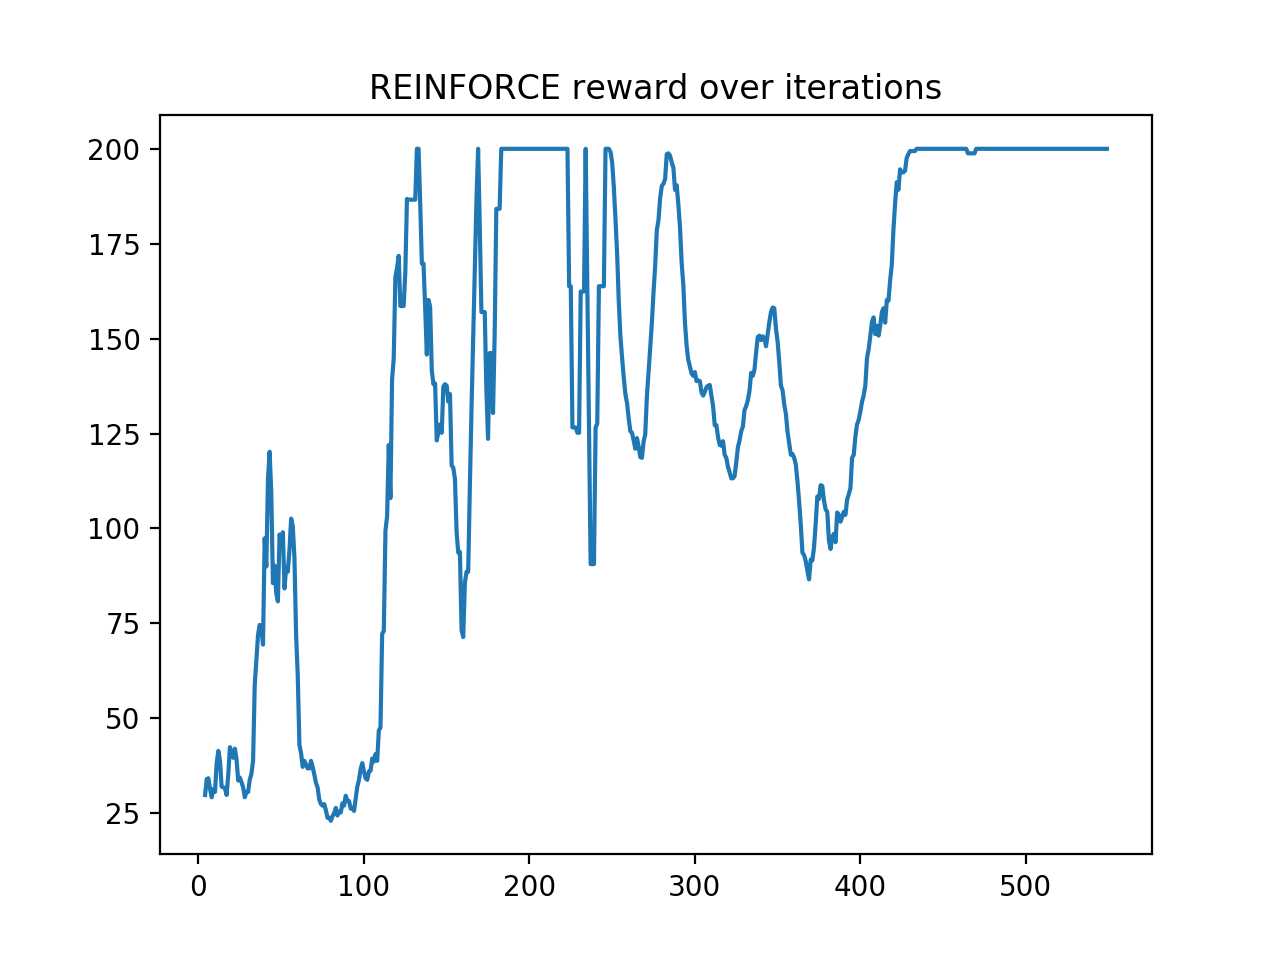
\includegraphics[width=\linewidth]{RF_conv.png}
  \caption{Convergence of the REINFORCE control}
  \label{fig:optPol1}
\end{figure}


Snippet of REINFORCE code:
\begin{figure}[h]
  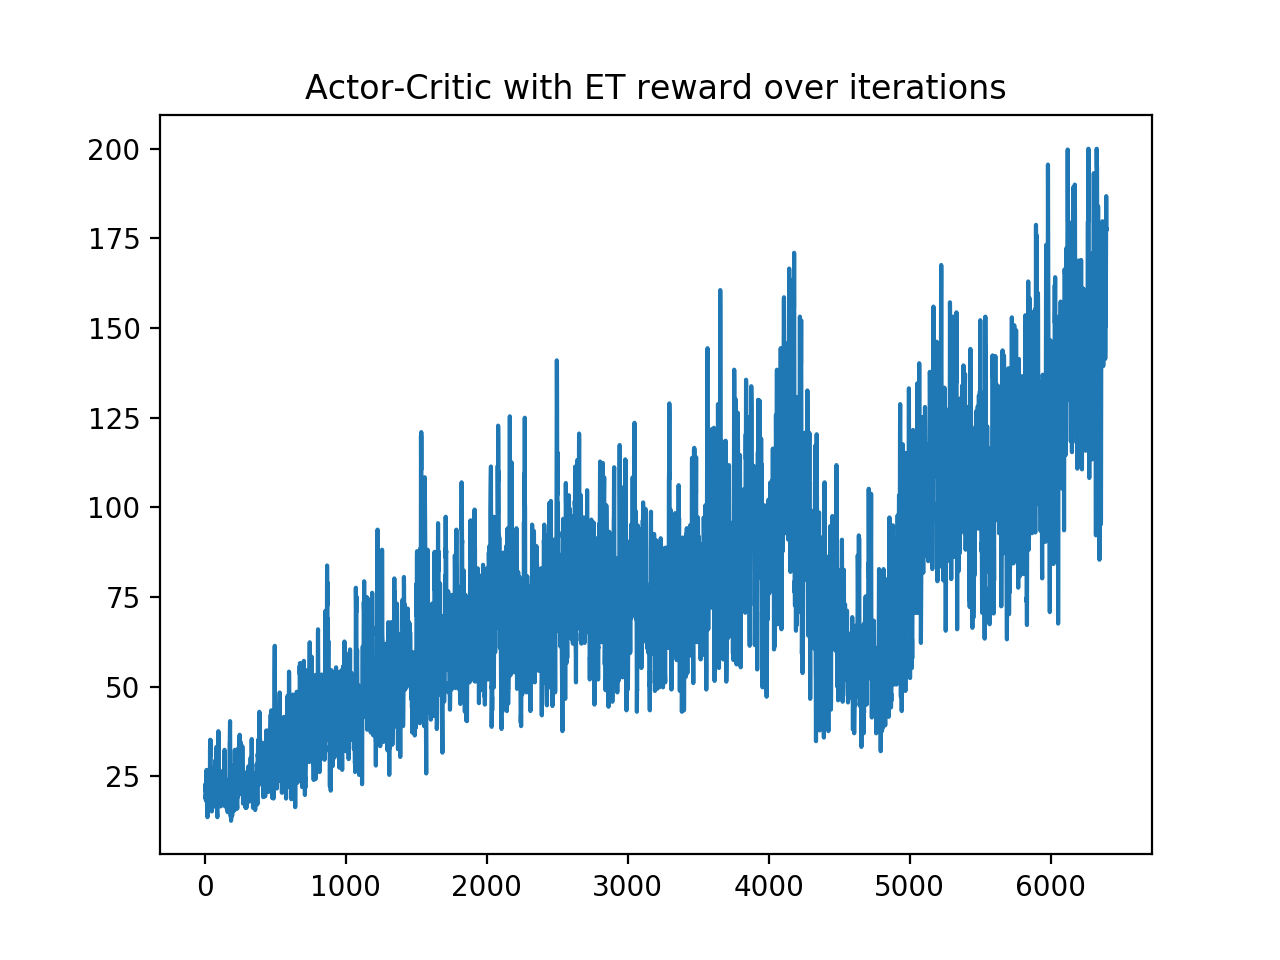
\includegraphics[width=\linewidth]{AC_conv.png}
  \caption{Convergence of the Actor Critic with Eligibility traces}
  \label{fig:optPol1}
\end{figure}

\begin{lstlisting}
def compute_loss(action_logprobs:tf.Tensor,returns:tf.Tensor) -> tf.Tensor:
    return -tf.math.reduce_sum(action_logprobs*tf.stop_gradient(returns))

def train_step(
    initial_state: tf.Tensor, 
    model: tf.keras.Model, 
    optimizer: tf.keras.optimizers.Optimizer, 
    gamma: float, 
    max_steps_per_episode: int) -> tf.Tensor:
  """Runs a model training step."""

  with tf.GradientTape() as tape:

    # Run the model for one episode to collect training data
    rewards, action_logprobs = get_episode(
        initial_state, model, max_steps_per_episode) 
    returns = get_expected_return(rewards, gamma)
    action_logprobs, returns = [
        tf.expand_dims(x, 1) for x in [action_logprobs, returns]] 
    loss = compute_loss(action_logprobs, returns)

  grads = tape.gradient(loss, model.trainable_variables)
  optimizer.apply_gradients(zip(grads, model.trainable_variables))
  episode_reward = tf.math.reduce_sum(rewards)
  return episode_reward
\end{lstlisting}

Snippet of Actor-Critic code:
\begin{lstlisting}
ef train_step(
    start_state: tf.Tensor, 
    ac_model: tf.keras.Model, 
    ac_optimizer: tf.keras.optimizers.Optimizer, 
    gamma: float, 
    max_steps_per_episode: int) -> tf.Tensor:
  """Runs a model training step."""
  state = start_state
  rewards = tf.TensorArray(dtype =tf.int32, size = 0, dynamic_size = True)
  gamma_tf = tf.constant(gamma)
  P_tf = tf.constant(1.0)
  lmd = 0.5
  lmd_tf = tf.constant(lmd)
  for t in tf.range(max_steps_per_episode):
    traces = [] 
    with tf.GradientTape() as tape:
      logits_actions, cval = ac_model(tf.expand_dims(state,axis = 0))
      action_sample = tf.random.categorical(logits = logits_actions,num_samples = 1)[0,0]
      action_logprob = tf.nn.log_softmax(logits_actions)[0, action_sample]
      next_state, reward, done = tf_env_step(action_sample)
      _, cval_next = ac_model(tf.expand_dims(next_state,axis = 0))
      td = tf.cast(reward,tf.float32)+gamma_tf*cval_next - cval
      a_loss = -action_logprob*tf.stop_gradient(td)*P_tf
      c_loss = huber_loss(tf.cast(reward,tf.float32)+gamma_tf*cval_next, cval)
      loss = a_loss+ c_loss
    grads_init = tape.gradient(loss, ac_model.trainable_variables)
    
    if len(traces) == 0:
      traces = [tf.zeros_like(grad_val, dtype = tf.float32)
                  for grad_val in grads_init]
    traces = [gamma*lmd_tf*tr + grad_val \
                for tr, grad_val in zip(traces, grads_init)]
    grads = [tf.reshape(td*tr,tr.shape) for tr in traces]

    ac_optimizer.apply_gradients(zip(grads, ac_model.trainable_variables))
    rewards = rewards.write(t, reward)
    if tf.cast(done, tf.bool):
      break
    state = next_state
    P_tf = P_tf*gamma_tf

  episode_reward = tf.math.reduce_sum(rewards.stack())
  return episode_reward
\end{lstlisting}

\end{document}
